\part{Annexos}

\pagestyle{annex1}
\chapter*{Annex 1 Codi de l'App}
\addcontentsline{toc}{chapter}{Annex 1 Codi de l'App}

El codi de l'app tot junt és el següent.

\begin{lstlisting}[language=Python, style=colorEX, caption=Codi sencer de l'App]
    # Importing packages

import tkinter as tk
import random
from tkinter import messagebox

# Begin and personalize window

class MemorizeApp:
    def __init__(self, root):
        self.root = root
        self.root.chapter("Memo App by Pol Sances")
        self.root.geometry("500x500")
        self.root.iconbitmap("Brain.ico")

    # Creating all the assets
        self.letters = self.generate_letters()

        self.label = tk.Label(self.root, text="", font=("Arial", 24))
        self.label.pack(pady=20)

        self.time_entry = tk.Entry(self.root, font=("Arial", 14))
        self.time_entry.insert(0, "Write time in seconds")
        self.time_entry.pack(pady=10)

        self.start_button = tk.Button(self.root, text="Start", command=self.start_memorize)
        self.start_button.pack(pady=5)

        self.answer_entry = tk.Entry(self.root, font=("Arial", 14))
        self.answer_entry.pack(pady=10)

        self.submit_button = tk.Button(self.root, text="Submit", command=self.check_answers)
        self.submit_button.pack(pady=5)

        self.reset_button = tk.Button(self.root, text="Reset", command=self.reset)
        self.reset_button.pack(pady=5)

        self.answer_entry.config(state="disabled")
        self.submit_button.config(state="disabled")
        self.reset_button.config(state="disabled")

        self.name = tk.Label(self.root, text="Made by Pol Sances Guirao", font=("Arial", 8))
        self.name.pack(pady=20)

     # Function to generate letters

    def generate_letters(self):
        letters = []
        for _ in range(20):
            letter = chr(random.randint(65, 90))
            letters.append(letter)
        return letters
    
     # Function to show letters with the time that user put in the time_entry textbox.

    def start_memorize(self):
        self.start_button.config(state="disabled")
        self.label.config(text="".join(self.letters))
        time_delay = int(self.time_entry.get()) * 1000  # Convert user seconds to milliseconds
        self.root.after(time_delay, self.show_entry)
        self.time_entry.pack_forget()  

     # Function to hide letters

    def show_entry(self):
        self.label.config(text="")
        self.answer_entry.config(state="normal")
        self.submit_button.config(state="normal")
        self.reset_button.config(state="normal")
        self.answer_entry.focus_set()

    # Function to check awnsers 

    def check_answers(self):
        user_answers = self.answer_entry.get().upper()
        correct_answers = "".join(self.letters)

        if user_answers == correct_answers:
            messagebox.showinfo("Result", "Correct answers!")
        else:
            messagebox.showinfo("Result", "Incorrect answers. Try again.")

        self.reset()

    # Reset function

    def reset(self):
        self.letters = self.generate_letters()
        self.answer_entry.delete(0, tk.END)
        self.label.config(text="")
        self.start_button.config(state="normal")
        self.answer_entry.config(state="disabled")
        self.submit_button.config(state="disabled")
        self.reset_button.config(state="disabled")
   

if __name__ == "__main__":
    root = tk.Tk()
    app = MemorizeApp(root)
    root.mainloop()

    \end{lstlisting}


La manera de fer funcionar l'app i el control de versions de github estan a \href{https://polsances13.github.io/roadto3bld/App.Html}{roadto3bld/App}.


\chapter*{Annex 2 Tutorial 3BLD}
\addcontentsline{toc}{chapter}{Annex 2 Tutorial 3BLD}
\pagestyle{annex2}
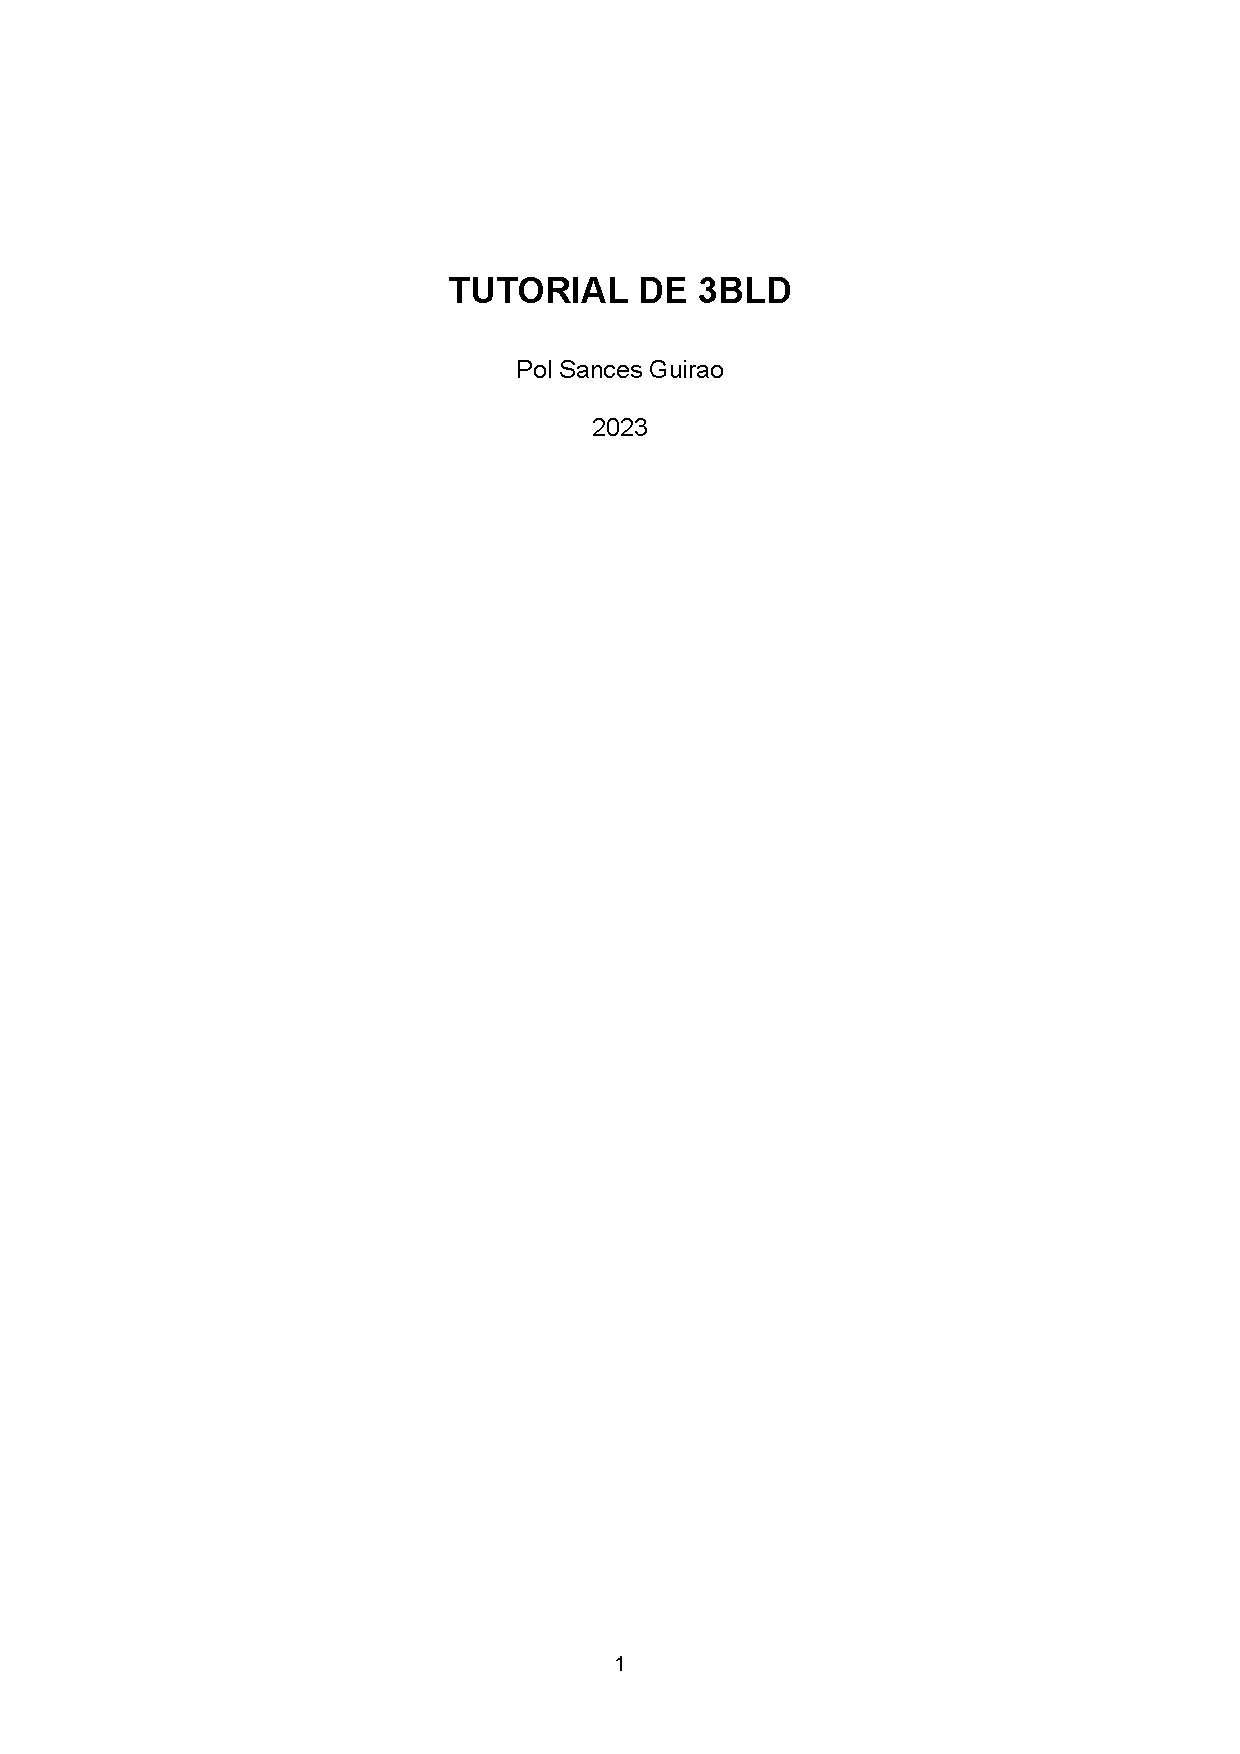
\includegraphics[width=\textwidth, page=1]{tutorial.pdf}
\includepdf[pages={2-13,23-24}, width=\textwidth, pagecommand={}]{tutorial.pdf}